\documentclass[../ClassicThesis.tex]{subfiles}
\begin{document}

%************************************************
\chapter{Classifiers / Klara}\label{ch:classifiers}
\newcommand{\TODO}[1]{\textcolor{red}{\\ \textbf{TODO:} #1 \\}}
%************************************************

\section{Classifiying idea}
In the previous chapters we covered the approach of solely finding plates within 3D-models. This approach needs the model to be very 'boxy'. Therefore sometimes the algorithm fails because of too many round edges or other noise. \\
This is why we tried another approach \cite{ransac} which is also being used by CGAL \cite{cgal}. We look for all kinds of primitive shapes in addition to plates. This allows us to split the model into separate objects which can then be independently converted to lasercutable plates. During the conversion we choose a specific method to realise this part with plates which often helps to achieve a more appropriate solution than to directly start finding plates. Due to the tolerance of the algorithm to noise we can even detect surface when there is a lot of texture.
Currently, our software system does not include the findings of the classifiers for a conversion. Instead we wanted to find out how well the algorithm works for our use case. \\
In order to properly include the classifiers we built up a theoretical structure to make the most of the findings. \\
A Classifier finds a particular shape like a plane, plate, box, sphere, cylinder, prism, etc. Classifiers can use findings of others for example the box finder depends on the previously found planes. As soon as all classifiers have finished their process all findings are hierarchichally grouped based on the depencies of the classifiers. Each finding is represented as a \emph{graphObject} which can either be of the type volume, like a box or cylinder for example, or a freeform. Freeforms are objects that could not be classified. But we check if this object is some kind of connector of volumes. This is valuable information for the conversion step because it means there needs to be something between specified volumes but this can be anything that the conversion method might choose. Then a graph is created which keeps all objects and their connections. Finally, the reconstruction starts. Volumes will be converted by its specific converter. For example a box converter. Connectors will result in plates which are connected to all volumes it belongs to. And from  unclassified objects we create plates based on the shapes found in this part of the mesh. \\
\*\\
% \paragraph{What is it usually used for? - pointclouds... which points do we intend to take for the algorithm?}
Usually, RANSAC is used with pointclouds. This means we need a lot of points and the more noise there is within the points the better for the algorithm. In our case we work with meshes where a model of a box might only have 8 points. This is a problem because the diagonals of the box look just like another plane to the algorithm because the sides and the diagonals are all supported by 4 points. 
On the other hand, when this box consisted of thousands of points they would all be somewhere on the sides. Meaning that the diagonal would not be found as a plane because it is maybe only supported by up to 10 points. In contrast, each side is supported by up to hundreds of points. Therefore, the RANSAC approach can definitely not be used in every case with any 3D-model. Instead it should be used as an additional way to split the model.
\section{RANSAC - Random Sample Consensus}
The RANSAC-approach firstly chooses a defined number of random points. These points are a minimal set from the point data and its number is defined by the shape which is being classified.\\
On the basis each of these minimal sets a candidate shape is generated and tested against all points in the data set. The candidate gets a score which tells how well the randomly chosen points represent the shape. This score can result from counting the points which lie within the candidate.\\
Based on this score a best model is saved or overwritten after several candidate attempts.
\section{Primitives}
In order to classify primitives a minimum number of points has to be defined which enable a reconstruction of the shape.
\subsection{Plane}
The minimal set for a plane are three points \{p1, p2, p3\} because three points uniquely identify a plane.\\
Once a plane candidate has been found it is necessary to check its plausibility. The deviations of the plane normal to the according point normals of p1, p2 and p3 should be less than an angle $\alpha$.\\
\*\\
After the detection of a best model it may be necessary to refit the candidate to all its inliers. We use the Least Squares method \cite{leastSquares}. We are aware that this method can only compute planes where its z-values are dependent on the x- and y-values which is not the case the the plane is perpendicular to the x-y-plane. Therefore we ignore planes to which this applies. Another possibility would be to work with eigenvectors where this would not be an issue.\\
When using the least squares method the problem can be transformed into an equation of the form Ax = b. Where A is a matrix consisting of the sum of all x values of the points, y values, x times y and x squared and y squared. \\

%sums
\begin{bmatrix}
\sum_{i=1}^m x_i^2 & \sum_{i=1}^m x_iy_i & \sum_{i=1}^m x_i\\
\sum_{i=1}^m x_iy_i & \sum_{i=1}^my_i^2 & \sum_{i=1}^m y_i\\
\sum_{i=1}^m x_i & \sum_{i=1}^m y_i & \sum_{i=1}^m 1
\end{bmatrix}
%
%coeffitients
\begin{bmatrix}
A\\
B\\
C
\end{bmatrix}
%
=
%
%solution
\begin{bmatrix}
\sum_{i=1}^m x_iz_i\\
\sum_{i=1}^m y_iz_i\\
\sum_{i=1}^m z_i
\end{bmatrix}


The least squares solution is the following plane equation: $z = Ax + By + C$.

\subsection{Cylinder}
The minimal set for a cylinder are two points \{$p_1, p_2$\}, see fig. \ref{fig:cylinder} for the reconstruction sketch. Those points are assumed to lie on the shell of the cylinder. The axis can be calculated by calculating the cross product of their normals $n_1$ and $n_2$. Based on the axis a projection plane is formed which is perpendicular to the axis. The two lines $l_1 = p_1 + x*n_1$ and $l_2 = p_2 + x*n_2$ are projected onto this plane and should have an intersection. If they do not intersect the candidate is invalid. Otherwise, the intersection point is marked as the center of the cylinder-candidate. The radius is the mean value of the distance of both points to the center on the axis.
\begin{figure}[!ht]
    \centering
    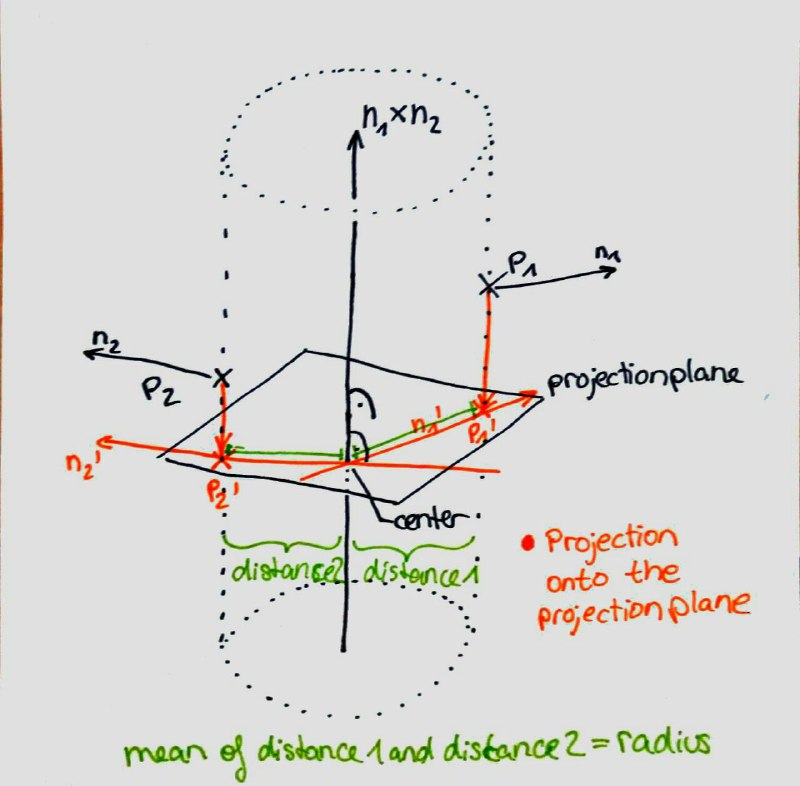
\includegraphics[width=\columnwidth]{Images/10-classifiers-cylinderClassification.jpg}
    \caption{Two points are enough to represent a cylinder. The axis can be reconstructed, as well as the radius.}
    \label{fig:cylinder}
\end{figure}

After a valid candidate has been formed we have to check the plausibility. For this we look for three indication. Firstly, the randomly chosen points p1 and p2 should not be the same, secondly, the calculated radius has to be larger than zero and lastly, the distances of the two points to the center should not exceed an epsilon value $\epsilon$.
\subsection{Prism - Dimitri}
\subsection{Other primitives}
In addition to the just mentioned objects any other primitive can be included in the search with RANSAC. \\
For this a number of minimum support points are needed. This number of points need to suffice to reconstruct the object. \\
Other points from the dataset can then be tested if they support the just constructed object. 
\section{Problems with non-pointcloud input}
In our usecase we do not have a pointcloud as input. Instead we operate on the much fewer points in a polygon mesh.\\
This has large influences on the threshold values that are used. The values taken from CGAL almost never achieved the desired results. We tried finding new values for any model which turned out to be infeasible. Therefore we tried adjusting the thresholds based on the number of vertices in the mesh or the volume of the bounding box. We have not encountered a working combination yet. This is a problem that needs to be tackled in future work.
\end{document}